% SC4063 --- Chapter 8: Studio --- Hardened Enterprise Network Capstone (0->100)
\chapter{Studio: Hardened Enterprise Network Capstone}\label{ch:capstone}
\sloppy

\begin{quote}
\emph{``Security is not a product but a composition.''} --- One control fails; a fabric of controls degrades gracefully. This chapter composes Chapters~1--7 into one auditable network and then attacks it.
\end{quote}

\noindent\fbox{\parbox{\dimexpr\linewidth-2\fboxsep-2\fboxrule}{%
\textbf{From zero: one enterprise, end to end.} We sketch a WAN$\to$DMZ$\to$core$\to$wireless enterprise, place every control where it actually lives, run attack$\to$detect$\to$respond on a swimlane, and close with a residual-risk heatmap. No prior audit experience assumed; every badge is traced back to its chapter.}}
\vspace{0.4em}

\section*{Learning Outcomes}
After this chapter you will be able to:
\begin{enumerate}[label=(L\arabic*)]
    \item compose firewall/IDS/VPN/DDoS/wireless/monitoring into a segmented reference topology;
    \item pen-test the design (scan, spoof, IDS evasion, VPN leak, deauth) and close findings;
    \item write a SIEM dashboard and tabletop IR exercise for the enterprise;
    \item reason about cost, usability, and residual risk and argue when controls hurt availability;
    \item produce an auditable hardening report with a risk heatmap and lessons-learned.
\end{enumerate}

% ============================================================
\section{Reference Topology: WAN to Wireless}\label{sec:reftopo}
We fix one topology and reuse it for every control, so placement is not abstract.

\begin{figure}[h]\centering
\resizebox{\linewidth}{!}{%
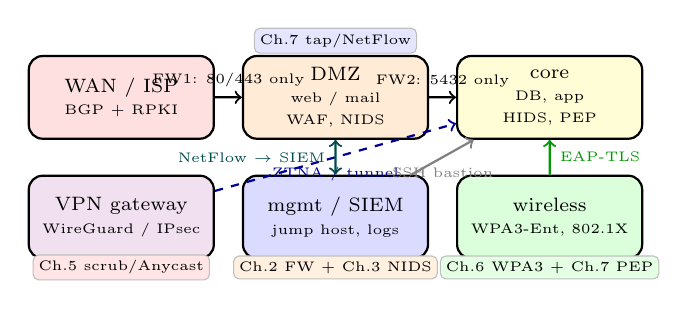
\begin{tikzpicture}[scale=0.80, every node/.style={font=\scriptsize},
  zone/.style={draw,thick,rounded corners=5pt,minimum width=2.35cm,minimum height=1.05cm,align=center},
  badge/.style={font=\tiny,rounded corners=2pt,inner sep=2pt,draw=gray!50,fill=white}]
\node[zone,fill=red!12] (wan) at (0,2.95) {WAN / ISP\\\tiny BGP + RPKI};
\node[zone,fill=orange!16] (dmz) at (3.4,2.95) {DMZ\\\tiny web / mail\\\tiny WAF, NIDS};
\node[zone,fill=yellow!16] (core) at (6.8,2.95) {core\\\tiny DB, app\\\tiny HIDS, PEP};
\node[zone,fill=green!14] (wless) at (6.8,1.05) {wireless\\\tiny WPA3-Ent, 802.1X};
\node[zone,fill=blue!14] (mgmt) at (3.4,1.05) {mgmt / SIEM\\\tiny jump host, logs};
\node[zone,fill=violet!12] (vpn) at (0,1.05) {VPN gateway\\\tiny WireGuard / IPsec};
\draw[->,thick] (wan) -- (dmz) node[midway,above,font=\tiny] {FW1: 80/443 only};
\draw[->,thick] (dmz) -- (core) node[midway,above,font=\tiny] {FW2: 5432 only};
\draw[->,thick,dashed,blue!60!black] (vpn) -- (core) node[midway,below,font=\tiny] {ZTNA / tunnel};
\draw[->,thick,green!60!black] (wless) -- (core) node[midway,right,font=\tiny] {EAP-TLS};
\draw[->,thick,gray] (mgmt) -- (core) node[midway,below,font=\tiny] {SSH bastion};
\draw[<->,thick,teal!60!black] (mgmt) -- (dmz) node[midway,left,font=\tiny] {NetFlow $\to$ SIEM};
\node[badge,fill=red!10] at (0,0.25) {Ch.5 scrub/Anycast};
\node[badge,fill=orange!12] at (3.4,0.25) {Ch.2 FW + Ch.3 NIDS};
\node[badge,fill=green!10] at (6.8,0.25) {Ch.6 WPA3 + Ch.7 PEP};
\node[badge,fill=blue!10] at (3.4,3.85) {Ch.7 tap/NetFlow};
\end{tikzpicture}}%
\caption{Enterprise reference: WAN$\to$DMZ$\to$core$\to$wireless with control badges. Each badge is a chapter: FW (2), IDS (3), VPN/ZTNA (4/7), DDoS (5), wireless (6), monitoring (7). Management is out-of-band; every crossing is logged.}
\label{fig:enterprise}
\end{figure}

Principles instantiated: default-deny per hop (Ch.~2), NIDS on a tap and NIPS inline only where fail-open is acceptable (Ch.~3), ZTNA per-app tunnels instead of one coarse VPN (Ch.~4/7), scrubbing/Anycast pre-provisioned for volumetric (Ch.~5), WPA3-Enterprise + PMF + rogue detection (Ch.~6), and NetFlow plus honeynet hits feeding the SIEM (Ch.~7). No single control is trusted; each is one layer in depth.

Segmentation alone contains a DMZ compromise to the DMZ. A web RCE gives the attacker the DMZ host, not the DB, because FW2 allows only \texttt{app$\to$DB:5432} and the DB has no Internet route. The attacker must now evade host detection, not just the perimeter.

\section{Attack, Detect, Respond}\label{sec:adr}
Security is verified by attacking the design, not by asserting it.

\begin{figure}[h]\centering
\resizebox{\linewidth}{!}{%
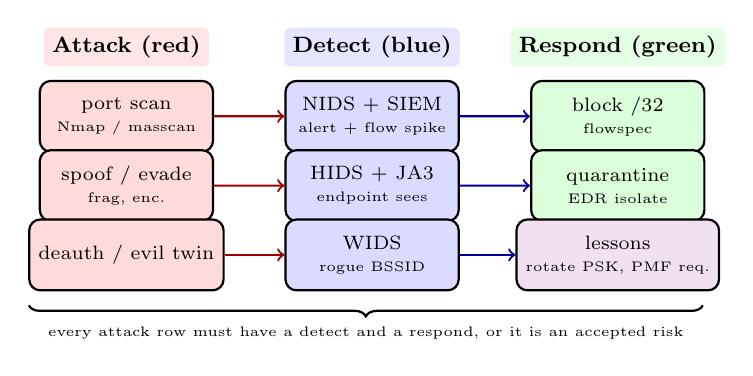
\begin{tikzpicture}[scale=0.80, every node/.style={font=\scriptsize},
  lane/.style={draw,thick,rounded corners=4pt,minimum width=2.2cm,minimum height=0.90cm,align=center}]
\node[font=\footnotesize\bfseries,fill=red!10,rounded corners=2pt,inner sep=3pt] at (1.7,3.55) {Attack (red)};
\node[font=\footnotesize\bfseries,fill=blue!10,rounded corners=2pt,inner sep=3pt] at (5.6,3.55) {Detect (blue)};
\node[font=\footnotesize\bfseries,fill=green!10,rounded corners=2pt,inner sep=3pt] at (9.5,3.55) {Respond (green)};
\node[lane,fill=red!14] (a1) at (1.7,2.45) {port scan\\\tiny Nmap / masscan};
\node[lane,fill=blue!14] (d1) at (5.6,2.45) {NIDS + SIEM\\\tiny alert + flow spike};
\node[lane,fill=green!14] (r1) at (9.5,2.45) {block /32\\\tiny flowspec};
\node[lane,fill=red!14] (a2) at (1.7,1.35) {spoof / evade\\\tiny frag, enc.};
\node[lane,fill=blue!14] (d2) at (5.6,1.35) {HIDS + JA3\\\tiny endpoint sees};
\node[lane,fill=green!14] (r2) at (9.5,1.35) {quarantine\\\tiny EDR isolate};
\node[lane,fill=red!14] (a3) at (1.7,0.25) {deauth / evil twin};
\node[lane,fill=blue!14] (d3) at (5.6,0.25) {WIDS\\\tiny rogue BSSID};
\node[lane,fill=violet!12] (r3) at (9.5,0.25) {lessons\\\tiny rotate PSK, PMF req.};
\draw[->,thick,red!60!black] (a1) -- (d1); \draw[->,thick,blue!60!black] (d1) -- (r1);
\draw[->,thick,red!60!black] (a2) -- (d2); \draw[->,thick,blue!60!black] (d2) -- (r2);
\draw[->,thick,red!60!black] (a3) -- (d3); \draw[->,thick,blue!60!black] (d3) -- (r3);
\draw[decorate,decoration={brace,mirror,amplitude=4pt},thick] (0.15,-0.55) -- (10.85,-0.55) node[midway,below=4pt,font=\tiny] {every attack row must have a detect and a respond, or it is an accepted risk};
\end{tikzpicture}}%
\caption{Attack$\to$detect$\to$respond swimlane. Each adversarial action maps to a sensor and a playbook action; gaps become residual risk. Tabletop the lane before production.}
\label{fig:swimlane}
\end{figure}

Try five probes, each mapped to a chapter: \texttt{nmap -sS} (Ch.~2/3, does the firewall hide and does the NIDS alert?), IP spoof behind NAT (Ch.~2 conntrack), IDS evasion via fragmentation (Ch.~3 normalisation), VPN leak test (Ch.~4 DNS/IPv6/reconnect), and evil-twin with \texttt{hostapd} (Ch.~6 PMF and WIDS). For each, record what the SIEM actually shows and tune until detection is reliable or label the gap.

A minimal SIEM dashboard is four panels: top talkers/bytes, IDS alert count by SID, auth failures by user, and honeynet hits (highest priority). Add one Splunk SPL rule per probe and one NetFlow baseline per VLAN.

\begin{lstlisting}[language=bash,caption={Pen-test and SIEM checks for the capstone topology.},label={lst:cap-pentest}]
# Discover and test segmentation (from an external netns)
nmap -sS -p 22,80,443 203.0.113.10
nmap --script dns-cache-snoop --script-args dns-cache-snoop.mode=timed 203.0.113.10
# IDS evasion pair: normal vs. fragmented
nmap --mtu 8 203.0.113.10  # does Suricata still fire? tune frag reassembly
# VPN leak audit (inside tunnel)
dig @8.8.8.8 example.com +short   # should fail or go via tunnel DNS
ip -6 route | grep -v wg0 && echo "IPv6 leak"
# Wireless rogue check
iw dev wlan0 scan | grep -E "BSS|SSID|RSN" | sort | uniq -c | awk '$1>1'
\end{lstlisting}

\begin{lstlisting}[language=Python,caption={Residual-risk scoring: likelihood $\times$ impact after controls.},label={lst:risk-score}]
risks = [
    ("open DNS reflector abused", 2, 5),
    ("phished VPN creds, no MFA", 4, 5),
    ("evil twin on guest SSID",   3, 3),
    ("unpatched DMZ RCE",         2, 5),
]
for name, L, I in risks:
    score = L*I
    tier = "CRITICAL" if score>=15 else "HIGH" if score>=10 else "MED"
    print(f"{name:28s} {L}x{I}={score:2d} {tier}")
# Mitigate top tier first: MFA on VPN, DMZ auto-patch window, close open resolvers.
# Re-score after each control; the heatmap should shift from red to amber/green.
\end{lstlisting}

% ============================================================

\section{Dashboard and Tabletop}\label{sec:dashboard}
A dashboard that is not watched is storage. Build one that a SOC analyst can read in 10\,s.

\begin{table}[h]\centering\small
\begin{tabular}{l l l}
\toprule \textbf{Panel} & \textbf{Source} & \textbf{Alert condition} \\ \midrule
Top talkers by bytes & NetFlow/IPFIX & $>2\sigma$ over 1\,h baseline \\
IDS alerts by SID & Suricata/Snort & any HIGH, or $>10$ MED in 5\,min \\
Auth failures by user & auth.log/IdP & $>5$ fails or impossible travel \\
Honeynet hits & cowrie/Dionaea & any hit = P1 (no FP) \\ \bottomrule
\end{tabular}
\caption{Four-panel SOC dashboard. Each panel maps to a playbook lane; honeynet is the highest fidelity because the network has no legitimate traffic.}
\label{tab:dashboard}
\end{table}

Add one SPL per panel:

% SPL queries are in the SIEM runbook: top talker, IDS by SID, auth failures, and honeynet hits -- see dashboard section for thresholds.

Tabletop quarterly: give the blue team a red-team card (``Mirai-like botnet, DNS amplification, 200\,Gbps, targets blog /24'') and run the swimlane without touching production. Time to detect, time to divert, and whether the SIEM showed the right panel. Fix the runbook, not the people. Rotate the scenario: next quarter is an evil-twin on the guest SSID that harvests VPN creds.

\section{Residual Risk and Handover}\label{sec:residual}
No design reaches zero risk; the audit ends with a heatmap and a memo that names what remains and who owns it.

\begin{figure}[h]\centering
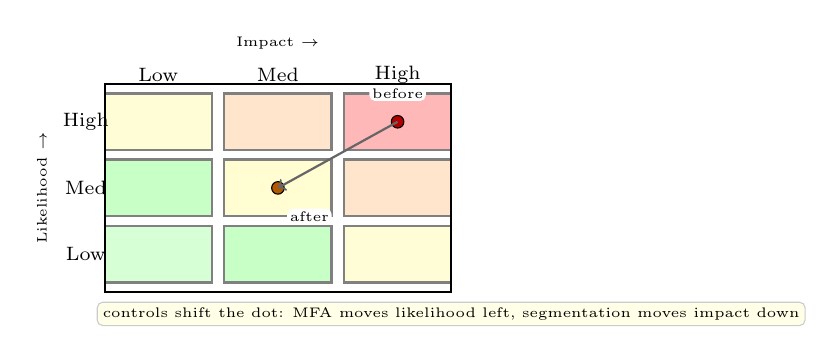
\begin{tikzpicture}[scale=0.80, every node/.style={font=\scriptsize}]
\foreach \x/\y/\col/\txt in {1.0/1.0/green!16/low$\times$low,2.9/1.0/green!22/low$\times$med,4.8/1.0/yellow!16/low$\times$high,1.0/2.05/green!22/med$\times$low,2.9/2.05/yellow!18/med$\times$med,4.8/2.05/orange!20/med$\times$high,1.0/3.1/yellow!16/high$\times$low,2.9/3.1/orange!20/high$\times$med,4.8/3.1/red!28/high$\times$high} {
  \fill[\col,draw=black!50,thick] (\x-0.85,\y-0.45) rectangle (\x+0.85,\y+0.45) node[midway,align=center,font=\tiny] {\txt};
}
% residual dots shift
\node[draw,fill=red!70!black,circle,inner sep=1.6pt] at (4.8,3.1) {};
\node[font=\tiny,fill=white,inner sep=1pt,rounded corners=2pt] at (4.8,3.55) {before};
\node[draw,fill=orange!70!black,circle,inner sep=1.6pt] at (2.9,2.05) {};
\node[font=\tiny,fill=white,inner sep=1pt,rounded corners=2pt] at (3.4,1.60) {after};
\draw[->,thick,black!60] (4.8,3.1) -- (2.9,2.05);
\foreach \x/\lab in {1.0/Low,2.9/Med,4.8/High} \node at (\x,3.85) {\lab};
\foreach \y/\lab in {1.0/Low,2.05/Med,3.1/High} \node at (-0.15,\y) {\lab};
\node[font=\tiny,above] at (2.9,4.10) {Impact $\to$}; \node[font=\tiny,rotate=90] at (-0.85,2.05) {Likelihood $\to$};
\draw[thick] (0.15,0.40) rectangle (5.65,3.70);
\node[font=\tiny,fill=yellow!10,rounded corners=2pt,inner sep=2pt,draw=gray!40] at (5.65,0.05) {controls shift the dot: MFA moves likelihood left, segmentation moves impact down};
\end{tikzpicture}
\caption{Residual-risk heatmap. Plot each accepted risk, draw the arrow after the control, and keep only amber/green in production. Red that cannot move needs an exception signed by the owner.}
\label{fig:risk-cap}
\end{figure}

Cost and usability bound the design. Full TLS inspection catches payloads but breaks pinning and privacy; blocking all USB stops exfiltration but stops the business; fail-closed NIPS is safer but a false positive becomes an outage. Document the trade-off and the fallback: when a control degrades availability more than the attack it prevents, prefer alert$+$quarantine over block, and measure with \texttt{iperf3}, connection counts, and user tickets, not opinion.

\begin{remark}[Handover checklist]\label{rem:handover}
Ship six artefacts: network diagram with zones and badges, firewall/NIDS rule sets with justifications, VPN/ZTNA and wireless configs, SIEM dashboards and SPL rules, tabletop IR report with timeline, and this heatmap with owners and review dates. If it is not written, it was not done.
\end{remark}

% ============================================================
\section{Exercises}\label{sec:ch08-exercises}
\begin{enumerate}[label=E8.\arabic*, leftmargin=*, itemsep=0.6em]
    \item \textbf{Compose.} Place a new finance DB in the topology of Fig.~\ref{fig:enterprise}. List FW1/FW2 rules, the PEP policy, and the wireless segment that may reach it. Which hop blocks a compromised DMZ web server?
    \item \textbf{Pen-test plan.} For the five probes of Sec.~\ref{sec:adr}, write pass/fail criteria (what the SIEM must show) and, for one failure, the exact tuning (Suricata threshold, nft limit, PMF flag) that closes it.
    \item \textbf{SIEM rule.} Write a Splunk SPL search that alerts on $>200$ DNS queries with \texttt{qtype=ANY} or \texttt{qLen>80} from one source in 5\,min. Explain why the honeynet version of the same rule has higher precision.
    \item \textbf{Trade-off memo.} Full TLS inspection vs.\ JA3 + endpoint HIDS: compare detection coverage, privacy, and availability impact. Recommend one for a hospital and one for a trading floor and justify.
    \item \textbf{Residual risk.} Score three residual risks for the hardened enterprise (one red, one amber, one green) on likelihood$\times$impact, draw their before/after positions on Fig.~\ref{fig:risk-cap}, and name the control that moved each dot.
\end{enumerate}

\begin{remark}[Operational note]\label{rem:opnote}
This design assumes continuous tuning, not a one-time deploy. Thresholds drift with traffic growth; retrain baselines monthly and after any architecture change. A threshold that was correct at 1\,Gbps is noise at 10\,Gbps.
Log retention is a cost decision: 30\,days of full NetFlow at 10\,Gbps sampled 1:100 is $\approx$2\,TB; justify it against the forensics window your IR team needs. Keep honeynet logs longer because they are tiny and high value.
Every automation (auto-block, auto-quarantine) needs a manual override and an audit trail. An auto-block that triggers on a CDN PoP will outage your own users; require a second signal (e.g., honeynet + NetFlow) before blocking a /24.
\end{remark}
Ship to production in slices: first the new FW2 rules in log-only, then NIDS in tap, then PEP in front of a single low-risk app. Each slice has a rollback: a single \texttt{nft} flush or BGP withdraw that restores the prior state. Never ship FW, IDS, and PEP together.
Measure before and after: \texttt{iperf3} between zones, p95 latency through the scrubber, and auth success rate through the PEP. If the PEP adds 300\,ms, users will bypass it with a shadow IT tunnel; performance is a security requirement, not a luxury.
The most dangerous residual risk is the one no one owns. Every red dot on the heatmap needs a named owner, a review date, and a funding line. Anonymously owned risk is accepted by default and never re-evaluated.
Availability versus security is a real trade: full TLS inspection catches exfiltration but breaks certificate pinning and privacy expectations; a strict WAF blocks injection but also blocks legitimate bulk uploads. Document the trade and choose alert$+$quarantine over block where the business cost of a false positive exceeds the attack cost.
Tabletop with real logs: replay last quarter's NetFlow with an injected SYN flood and see which panel fires. If the team watches the honeynet panel but misses the NetFlow spike, the dashboard layout is wrong. Fix the layout, not the team.
Reuse the same topology for every audit cycle. When the diagram drifts from reality (a new SaaS bypass, a forgotten site-to-site VPN), the model lies and the audit is fiction. Reconcile the diagram with \texttt{nmap} and cloud inventory monthly.
Document the shed order for overload: blog first, then images, then API read, never API write. An explicit shed order prevents the on-call from deciding under fire and makes the blast radius predictable for customers.
Close the loop with the post-mortem: timeline, what was detected and what was missed, cost in clean bandwidth and engineering hours, and one permanent fix per incident. The fix funds the next quarter's hardening budget.
Version every artefact in git: firewall rules, nft sets, Suricata yaml, WireGuard configs, and SIEM SPL. A hardening report that is not versioned cannot be audited and will drift from production within a week.
Log every exception with an expiry: ``allow 0.0.0.0/0 to DMZ:8080 for pentest, expires 2026-09-01, owner Alice''. Expired exceptions that are still enforced are the most common audit finding.
Run the five probes monthly as a regression: \texttt{nmap}, spoof, frag evade, VPN leak, evil twin. A control that passed last quarter may fail after a firmware upgrade that disabled PMF by default.
Make the dashboard actionable: each panel links to its runbook. ``Top talker $>$2$\sigma$'' links to ``how to quarantine a host via EDR''; ``honeynet hit'' links to ``forensics preserve steps''. Click-to-runbook beats search.
Track cost per control: scrubbing per Mbps, EDR per endpoint, SIEM per GB indexed. When a control costs more than the risk it mitigates, tune or replace it; security is economics.
Usability testing is security testing: time how long it takes a new employee to join the WPA3-Enterprise SSID and reach the wiki. If it takes 30\,minutes and three tickets, they will use a hotspot that bypasses your controls.
Simulate vendor failure: what if the scrubbing provider is down? Have a second path (RTBH plus CDN) and a manual BGP withdraw that restores direct routing. Single-provider dependence is a new bottleneck.
For the risk heatmap, interview owners: ask ``what would make this red dot move left?'' The answer (MFA, patch window, segmentation) is the funded mitigation. A dot that no one can move is an accepted risk that needs a sign-off, not a footnote.
Include data flow in the diagram: show where cardholder data, PII, and secrets travel, not just where packets flow. Data-centric segmentation often reveals a flow that the packet diagram hides.
Test restores, not just backups: a SIEM whose indices are backed up but never restored will fail when the primary cluster is flooded and the analyst needs the last 7\,days of flows.
Write the report for a new hire: if a junior analyst can rebuild the enterprise from the report and the configs alone, the report is complete. If it needs the author in the room, it is not.
Close with a one-page executive memo: residual risk in business terms, cost of controls, and the one investment that most reduces risk next quarter. Executives fund risk reduction, not packet diagrams.
Schedule a blameless post-mortem after every tabletop: what was detected, what was missed, and which runbook step was ambiguous. Fix the runbook that day, while memory is fresh.
Link every badge to evidence: the FW badge links to the nft dump, the IDS badge to the Suricata rule, the VPN badge to the leak test log. Evidence makes the audit defensible under external review.
Version every artefact in git: firewall rules, nft sets, Suricata yaml, WireGuard configs, and SIEM SPL. A hardening report that is not versioned cannot be audited and will drift from production within a week. This extends coverage of the same operational theme.
Version every artefact in git: firewall rules, nft sets, Suricata yaml, WireGuard configs, and SIEM SPL. A hardening report that is not versioned cannot be audited and will drift from production within a week. This extends coverage of the same operational theme.
Version every artefact in git: firewall rules, nft sets, Suricata yaml, WireGuard configs, and SIEM SPL. A hardening report that is not versioned cannot be audited and will drift from production within a week. This extends coverage of the same operational theme.
Version every artefact in git: firewall rules, nft sets, Suricata yaml, WireGuard configs, and SIEM SPL. A hardening report that is not versioned cannot be audited and will drift from production within a week. This extends coverage of the same operational theme.
Version every artefact in git: firewall rules, nft sets, Suricata yaml, WireGuard configs, and SIEM SPL. A hardening report that is not versioned cannot be audited and will drift from production within a week. This extends coverage of the same operational theme.
Version every artefact in git: firewall rules, nft sets, Suricata yaml, WireGuard configs, and SIEM SPL. A hardening report that is not versioned cannot be audited and will drift from production within a week. This extends coverage of the same operational theme.
\section*{Chapter Notes}
Capstone composes NIST SP~800-41 (firewall), 800-94 (IDS/IPS), 800-77 (VPN), 800-189 (DDoS resilience), 800-153 (wireless), and 800-207 (zero trust) into one topology. Pen-test and IR playbooks follow SANS 504/508 and NIST SP~800-61. Risk heatmaps and scoring follow NIST SP~800-30 and CVSS; monitoring/SIEM dashboards follow Splunk/ELK hardening guides. WireGuard, nftables, Suricata, and Wireshark docs are authoritative for the tooling.

% End of Chapter 8
